\documentclass[11pt,notitlepage]{article}
\usepackage[margin=1in]{geometry}
\usepackage{epsfig}
\usepackage{subfigure}
\usepackage{amsmath}
\usepackage[usenames,dvipsnames,svgnames,table]{xcolor}
\usepackage{amssymb}
\usepackage{setspace}
\usepackage{graphicx} % Include figure files
\usepackage{times}
\usepackage{amsthm}
\usepackage[numbers,sort&compress]{natbib}
\usepackage{hyperref}
\hypersetup{bookmarks=true, unicode=false, pdftoolbar=true, pdfmenubar=true, pdffitwindow=false, pdfstartview={FitH}, pdfcreator={}, pdfproducer={}, pdfkeywords={} {} {}, pdfnewwindow=true, colorlinks=true, linkcolor=red, citecolor=Green, filecolor=magenta, urlcolor=cyan,}
\usepackage{authblk}
\usepackage{bbm}
\usepackage{algorithm}
\usepackage{algpseudocode}
\newtheorem{proposition}{Proposition}
 
\usepackage{parskip}
 
\newcommand{\lod}{\text{LOD}}
\newcommand{\varr}{\text{Var}}
 
\newcommand{\dan}[1]{\textcolor{blue}{#1}}
\newcommand{\vlr}[1]{\textcolor{red}{#1}}

\newcommand{\numpeople}{M}
\newcommand{\numdays}{N}
\newcommand{\samplematrix}{\mathbf{A}}
\newcommand{\samplematrixentry}{A}
\newcommand{\incidence}{c}
\newcommand{\assaycost}{\sigma}

\newcommand{\li}{\ell_i}
\newcommand{\lo}{\ell_0}

\newcommand{\prob}{\mathbb{P}}
\newcommand{\expec}{\mathbb{E}}

 
\begin{document}
%%%%%%%%%% Authors
\author[1]{\vlr{Violet Ross}\thanks{violet.ross@colorado.edu}}
\author[1,2,3]{\dan{Daniel B. Larremore}\thanks{daniel.larremore@colorado.edu}}
\affil[1]{Department of Computer Science, University of Colorado Boulder, Boulder, CO 80309 USA}
\affil[2]{BioFrontiers Institute, University of Colorado Boulder, Boulder, CO 80303 USA}
\affil[3]{Santa Fe Institute, Santa Fe, NM 87501 USA}
%%%%%%%%%% Suppress Date
\date{}
%%%%%%%%%% Title
\title{Title}
\maketitle
%%%%%%%%%% Abstract
\begin{abstract}
abstract
\end{abstract}
%%%%%%%%%% Content


    %%%    
    %%%   
  %%%%%%%
   %%%%%
    %%%
     %

\section{Background}
\label{sec-intro}

Viral kinetics, changes in the concentration of virus within an infected individual over time, were first modeled in the 1990s, for the study of HIV \cite{perelson1996hiv}.
Since then, viral kinetics (VK) models have proved useful for a variety of tasks.
VK modeling can be used to address clinical questions, such as explaining why recipients of a new hepatitis C treatment exhibited high rates of drug-resistance \cite{rong2012modeling}, as well as epidemiological questions, such as determining optimal testing and isolation strategies for population-level management of SARS-CoV-2 \cite{kissler2021viral}.  
Modeling viral kinetics also allows us to understand how infections with the same virus might vary depending factors such as the variant \cite{russell2024combined}, the vaccination status of the host \cite{ke2022longitudinal}, whether the host has been infected before \cite{kissler2023viral}, and demographic characteristics of the host, such as age \cite{russell2024combined}.

A fundamental challenge of building VK models is the amount and type of data needed, and the cost associated with collecting it.
If too few samples are collected, the model will struggle to accurately estimate the dynamics of viral concentration, producing poor estimates of epidemiological parameters.
Collecting large numbers of samples presents its own challenges, increasing discomfort for subjects and incurring high costs for the investigator \cite{canini2011viral}.   

Data for fitting VK models may be collected via a challenge study or from naturally occurring infections.
Challenge studies produce high-quality data, but typically use a controlled dose of a less agressive strain of the pathogen being studied, and are not carried out for newly emergent pathogens.
Serial sampling after symptom onset or a positive test result captures naturally occurring infections.
The participants in serial sampling either have confirmed cases prior to recruitment or share a household with someone who has a confirmed case.
Studying the former set of participants, called a reactive clinical cohort, results in data with systematically undersampled proliferation phases.
Sampling from the latter group, a case-ascertained household cohort, can produce data that captures the proliferation phase, but still conditions on the fact that the index case experienced a severe enough infection to seek care, biasing down-the-line analysis.
Naturally ocurring infections can also be captured by sampling from a community-based longitudinal cohort, a group of individuals from a shared community who are sampled repeatedly over an extended period of time with the intention of capturing complete infections as they occur.
This approach, as it has been implemented thus far [CITE], has the highest sampling and assaying costs, recording viral concentrations from all participants at a high frequency over an extended period of time.
Though this approach has been costly, it has also produced excellent data for building VK models [CITE].

Gold-standard data for VK modeling emerged as a result of surveillance efforts during the SARS-CoV-2 pandemic, enabling an influx of VK modeling research which was crucial to improving understanding of the pathogen and making public health decisions [CITE, CITE, CITE].
This data was collected from a community-based longitudinal cohort.
Existing data that has been collected from as many participants and with as much frequency as the COVID-era data is rare.
We aim to build VK models that are as accurate as those built on the extensive COVID surveillance data — without requiring costly data collection.
Optimal design for VK modeling has been explored in previous work — Canini and Carrat investigated the optimal number of participants, number of samples per participant, and temporal distribution of these samples for fitting a mechanistic model of influenza \cite{canini2011viral}.
\vlr{Other work on efficient sampling for building viral kinetics has explored...} \cite{}.

% To optimally identify infections in a population, our approach employs sample pooling. 
% Sample pooling was first proposed by Robert Dorfman as a strategy for syphilis screening in the United States military during World War II. 
% The limit of detection for many assays is often far lower \vlr{[HOW MUCH]} than the amount of virus in a single positive sample. 
% This fact is the basis of sample pooling — combining several samples into a ``pool'' and then testing the pool using a single assay.
% If the pool is negative, all of its constituent samples are negative.
% If the pool is positive, at least one of the samples within it is positive.
% Several approaches optimized for varying criteria have been proposed for determining which of the samples in a positive pool are themselves positive \cite{furstenau2020sample}.
% Though Dorfman's design was never employed during the war, it has proved useful since then for providing diagnostic results using less reagant and with a faster turnaround time, as well as reducing the cost associated with obtaining population-level prevelance estimates \cite{grobe2021sample}.

We propose an adaptive approach to fitting a generalized phenomonological model of viral kinetics that is optimal with respect to number of assays used.
This approach consists of three main stages.
In the first stage, we use pooling to indentify individuals in the cohort who do not experience infection with the pathogen of interest during the window of sampling.
In the second stage, we use prior knowledge of typical infection durations to efficiently find infections in particpant-time space.
In the third stage, we use an active learning approach to fit a phenomonological VK model, maximizing information gain while minimizing assay costs.
We fit a two-phase piecewise linear model of VK with parameters drawn from a Bayesian hierarchical model, an approach which has been used to model viral kinetics in work on SARS-CoV-2 \cite{kissler2023viral} and \vlr{other viruses} \cite{}.

\section{Parameterization}
The typical output of a quantitative polymerase chain reaction (PCR) assay is the cycle threshold.
The cycle threshold (Ct) of a sample is the number of amplification cycles needed for the virus to be detected.

We seek to model the viral RNA concentration of samples over time.
Viral RNA concentration can be used to describe or estimate information like viral load and infectiousness \cite{?}.
The cycle threshold of a sample is roughly the negative logarithm of the viral RNA concentration \cite{?}.
The limit of detection (LOD) of an assay is the viral RNA concentration below which samples will be identified as negative.
For many infectious agents, viral RNA concentration increases during proliferation and decreases during clearance approximately exponentially.
This corresponds to a two-phase linear model of Ct with negative slope during proliferation and positive slope during clearance.
For simplicity, we model the value of the positive logarithm of viral RNA concentration over time.
However, this value can easily be converted to the cycle threshold or the concentration of viral RNA.

Our viral kinetics models will specify the value of $\omega$ (the logarithm of the amount by which viral RNA concentration exceeds zero) over time $t$.
When the viral RNA concentration is less than the LOD, $\omega$ is equal to 0.
Letting $\omega$ be the difference of viral concentration and LOD allows us to omit LOD from our equations.

Observed values of $\omega$ increase linearly with $t$ until a peak value is reached and then decrease linearly with $t$.
Two-phase (or segmented) regression is often used to fit models to data of this shape \cite{?}.
A traditional parameterization of the two-phase linear model uses four parameters, a y-intercept $\alpha$, two slopes $\beta_1$ and $\beta_2$, and a breakpoint $\psi$ that specifies the time of peak concentration.
When modeling viral kinetics, the value of $\alpha$ is simply equal to the LOD, so that $t = 0$ is the beginning of detectable infection.
The equation for $\omega$ is
\begin{equation*}
    \omega(t) = \beta_1 t + \beta_2 t \mathbbm{1}\{t > \psi\}.
\end{equation*}
A depiction of the tent function is given in Figure \ref{?}.

\vlr{fig of tent func here}

The two-phase linear model (sometimes called the ``tent function'') only learns from positive values.
If the infected period is densely sampled, this may be an appropriate choice of parameterization.
However, when we have only a small number of samples from the infected period, negative assay results can provide valueable information (as we will see in Section \ref{?}) 

For empirical data, $\omega$ values are shaped like a tent only during detectable infection, outside of which they are all 0.
The following model accounts for the pre- and post-infection periods:
\begin{equation}\label{eqn:calendar-witch}
    \omega(t) =
        \begin{cases}
            0 & t < \psi_1 \\
            (t - \psi_1) \frac{V}{\psi_2 - \psi_1} & \text{if } \psi_1 \leq t < \psi_2 \\
            V - (t - \psi_2) \frac{V}{\psi_3 - \psi_2}   & \text{if } \psi_2 \leq t < \psi_2 \\
            0 & \psi_3 \leq t.
        \end{cases}
\end{equation}
The three $\psi$ parameters are used to indicate the boundaries of the pre-infection period, the proliferation phase, the clearance phase, and the post-infection period.
This parameterization enables learning from negative test results, but the parameters are not interchangeable over an ensemble of infections.
For instance, if we fit two empirical trajectories to Equation \ref{eqn:calendar-witch} that are identical, but occured over different time periods, the values of the $\psi$ parameters would be different for each.

We therefore change our parameterization so that for all infections, the time of peak viral load is 0.
Then the model is given by
\begin{equation}\label{eqn:reindex-witch}
    \omega(t) =
        \begin{cases}
            0 & t < \psi_1 \\
            V(t + \frac{t}{\Delta_p}) & \text{if } -\Delta_p \leq t < 0 \\
            V(1 - \frac{t}{\Delta_c})   & \text{if } 0 \leq t < \Delta_c \\
            0 & \Delta_c \leq t.
        \end{cases}
\end{equation}
Here, $\Delta_p$ is the duration of the duration of the proliferation phase and $\delta_c$ is the duration of the clearance phase.
This is the parameterization we employ.

\begin{figure}
    \centering 
    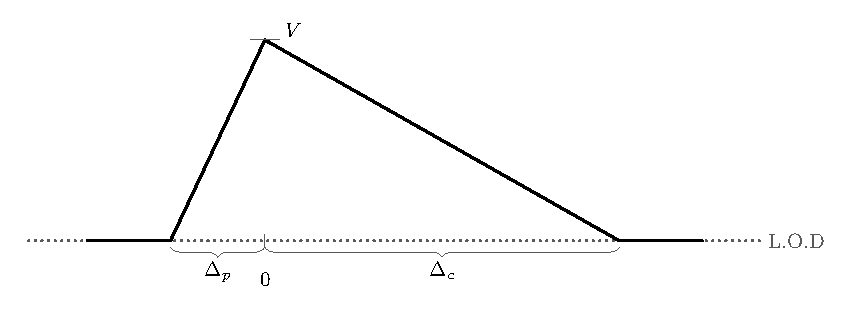
\includegraphics[width=1\textwidth]{witch_hat_diagram.pdf}
    \caption{The function $\omega(t)$.}\label{fig:witch}
\end{figure}

A plate diagram for our Bayesian hierarchical model (BHM) is given by Figure \ref{fig:bhm}.
In this BHM, each infection $i$ has its own parameters $V^{(i)}$, $\delta_p^{(i)}$, and $\delta_c^{(i)}$, each of which is drawn from a population-level distribution with center and spread $\mu$ and $\sigma$.
The population-level distributions are positive and non-centered \cite{?}.
An observation from an infection at time $t$ is drawn from a normal distribution centered at $\omega(t)$ with standard deviation $\sigma_\epsilon$.
Each infection also has a parameter $\psi^{(i)}$ which is used to reindex the data so that it is approximately centered at the peak of the infection.
For each infection, $\psi^{(i)}$ is drawn from a distribution that is weakly centered at the \vlr{[decide here: center of interval or highest observed viral concentration?]}



\begin{figure}
    \centering 
    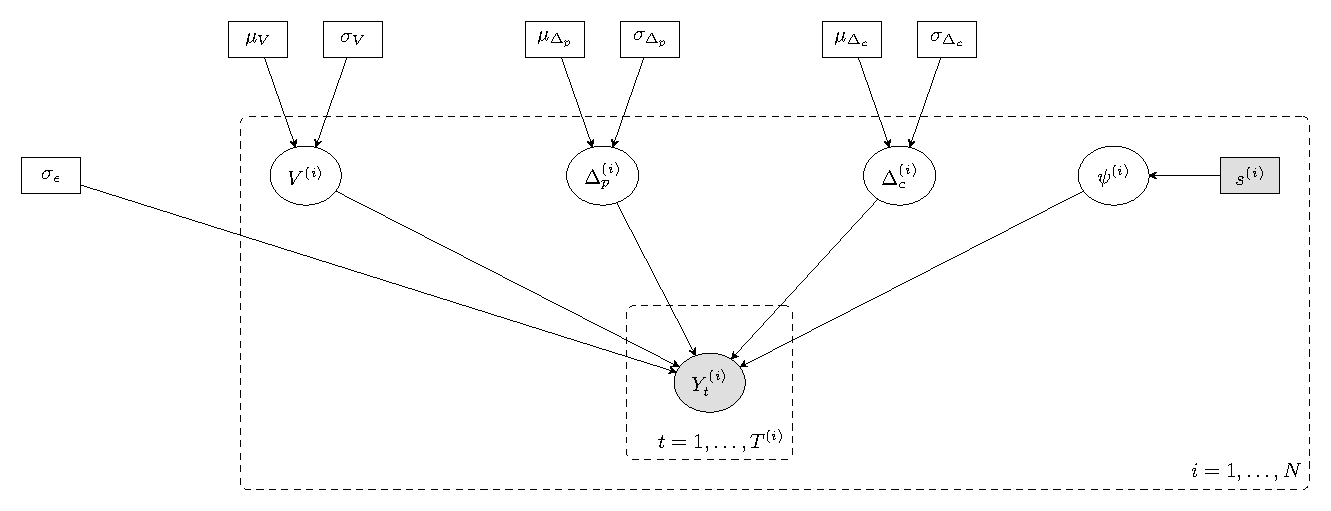
\includegraphics[width=1\textwidth]{plate_diagram_witch.pdf}
    \caption{The Bayesian hierarchical model.}\label{fig:bhm}
\end{figure}

\section{Study Design and Optimized Assay Approaches}
We develop methods for fitting a viral kinetics model given a set of \vlr{(is there a word more general than "saliva" that I can use here?)} samples collected from $\numpeople$ individuals over $\numdays$ days.
These samples can be arranged into an $\numpeople$ by $\numdays$ matrix $\samplematrix$, where an entry $\samplematrixentry_{i,j}$ is the sample collected from participant $i$ on day $j$.
We say that $\samplematrixentry_{i,j} > 0$ if individual $i$ had viral RNA concentration above the limit of detection (LOD) of our assay on day $j$.
Otherwise, $\samplematrixentry_{i,j} = 0$. 
Observing the value of an entry in the matrix amounts to assaying the corresponding sample.

Data of this kind might emerge in a variety of ways.
Samples originally collected for a study focusing on one pathogen can be arranged into this format and used to fit a model of another pathogen.
\vlr{(Need another example of where this data might come from.)}
Of course, researchers might collect samples from a population with the express purpose of employing the assaying approaches proposed here.

The ultimate goal of this work is to develop efficient algorithms to obtaining a fit model of the viral kinetics of a pathogen, starting from the matrix $\samplematrix$ whose values we have not yet observed. 
There are two main types of algorithms we propose towards this end: the first locates infections within the sample matrix and the second fits a viral kinetics model to those infections.

Unless researchers specifically target individuals who they know are likely to become infected within a fixed period of time (an approach which incurs its own high expenses), $\samplematrix$ will be a sparse matrix.
If we were to assay every sample in $\samplematrix$, most of the results will be negative, offering little information to our model.
That is, only a small proportion of the assays perfomed in the complete assaying case are informative.
This suggests that we can locate the infections within $\samplematrix$ using far fewer than the $\numpeople * \numdays$ assays required by the complete testing approach.
But how many tests are actually needed, and how should we distribute them among the samples?

\subsection{Infection Discovery}
The problem of infection discovery amounts to identifying continuous sequences of positive entries within the rows of $\samplematrix$.
We need not record the entire infection from start to finish, but rather identify at least one of the positive values within it.
This can be achieved by the following algorithm.

Suppose you are given the matrix $\samplematrix$ with unobserved entries and cumulative incidence $\incidence$.
Assume that the duration of each infection $\li$ is drawn from some continuous positive distribution with practical lower bound $\lo$ such that $\prob(\li < \lo) < \alpha$ for some small constant $\alpha$.
\vlr{(how are we doing this in sims since we're working in discrete time?)}

The algorithm proceeds as follows. \vlr{(a diagram might be useful for this)}
Within each row: pool the samples and apply a single assay to the pool \vlr{(gotta show that we'll stay above LO)}. 
For each row $i$ on which the assay returns a negative result, set $\samplematrixentry_{i,j} = 0$ for all $j$.
This row does not contain an infection and can now be removed from consideration.
For each row $i$ on which the assay returned a positive result, individually assay entries at an interval of $\lo$.
That is, assay samples $\samplematrixentry_{i,0}, \samplematrixentry_{i,\lo}, \samplematrixentry_{i,2\lo}, \samplematrixentry_{i,3\lo}, \dots$. 

Both the accuracy of this approach and the cost reduction it offers can be expressed in closed form.
We quantify the accuracy of the infection discovery algorithm by the probability that an arbitrary trajectory is not missed.
An infection is missed if none of the samples taking during its duration are assayed by the algorithm.
The probability that an arbitrary infection $i$ is missed by the infection discovery algorithm is described by the inequality
\begin{equation}\label{eqn:miss}
    \prob(\text{miss } i) < \alpha - \frac{\alpha}{\lo} \expec \left[ \li | \li < \lo  \right]
\end{equation}
The cost $C$ of running the infection discovery algorithm over matrix $\samplematrix$ is 
\begin{equation}\label{eqn:cost}
    C = \numpeople \numdays (\frac{1}{\numdays} + \frac{c}{\lo}).
\end{equation}
This reduces the cost of the brute force approach by a factor of $(\frac{1}{\numdays} + \frac{c}{\lo})$.
Infection discovery gets cheaper as the number of individuals sampled increases and the ratio of the cumulative incidence to the sampling interval decreases.
Derivations for Equations \ref{eqn:miss} and \ref{eqn:cost} can be found in Section \ref{sec:infx-disc}.

We fit the BHM to the data obtained from infection discovery using the Stan statistical software, which performs Hamiltonian Monte Carlo.

\begin{figure}
    \centering 
    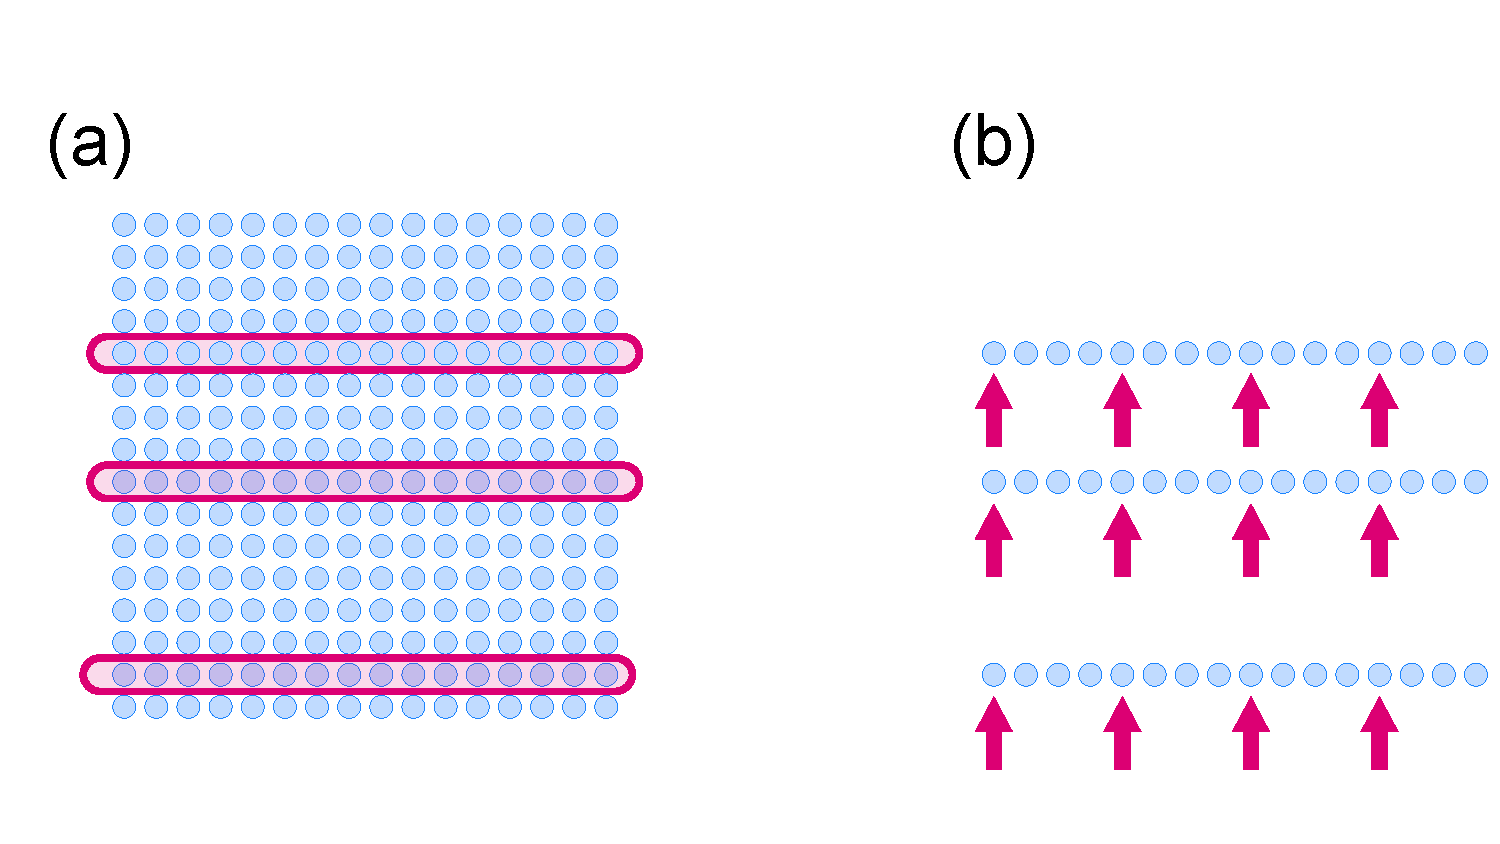
\includegraphics[width=1\textwidth]{../fig/infection_discovery_fig.pdf}
    \caption{Diagram of the infection discovery process. 
    Panel (a) illustrates the sample pooling phase and Panel (b) illustrates the interval sampling phase.} \label{fig:infection-discovery}
\end{figure}

\subsection{Adaptive Sampling}
The BHM can also be fit via adpative sampling.
The general framework is to perform infection discovery, fit the model, use that fit to select which samples to assay next, and fit again.
The assay-fit cycle can be performed iteratively, at the cost of reagants and both laboratory and computational time.

The central choice in designing the adaptive sampling approach is the choice of acquisition function.
Our adaptive sampling algorithm assays at the timestamp which maximizes the differential entropy of the posterior predictive.
Let $\theta^{(i)} = (V^{(i)} , \Delta_p^{(i)}, \Delta_c^{(i)}, \phi^{(i)}, \sigma_\epsilon)$ be the vector containing the infection-level parameters for infection $i$, along with $\sigma_\epsilon$.
The posterior predictive distribution, $p(y_t^{(i)} | \{y\})$, computes the probability that the observed value of infection $i$ at time $t$ is $y_t^{(i)}$, given all observations in the observed data.
Then $p(y_t^{(i)} | \{y\}) = \int_{\theta^{(i)}} P(y_t^{(i)} | \theta^{(i)})P(\theta^{(i)} | \{y\}) d\theta^{(i)}$ which can be computed by numerical integration over the draws produced by HMC.

Then the differential entropy $H(y_t^{(i)} | \{y\})$ of the posterior predictive distribution at $y_t^{(i)}$ is given by
\begin{equation*}
    H(y_t^{(i)} | \{y\}) = \int_{-\infty}^{\infty} p(y_t^{(i)} | {y}) \log \frac{1}{p(y_t^{(i)} | {y})} dy_t^{(i)}.
\end{equation*}
This value is also computed by numerical integration.
The acquisition function assays, for each infection, the un-assayed sample whose timestamp maximizes $H$.
If $H$ is maximized at multiple samples, one is chosen uniformly at random.

The adaptive sampling process proceeds as specified in Algorithm \ref{alg:adaptive}, returning the final fit $\Theta$.

\begin{algorithm}
\caption{Adaptive sampling}\label{alg:adaptive}
\begin{algorithmic}[1]   % [1] numbers every line
    \State $\text{data} \gets$ \Call{infection\_discovery}{$M$}
    \State $\Theta \gets$ \Call{HMC}{\text{data}}
    \While{stop $=$ False}
        \State $\text{data} \gets$ \Call{acquisition\_function}{data, $\Theta$}
        \State $\Theta \gets$ \Call{HMC}{\text{data}}
    \EndWhile
    \State \Return $\Theta$
\end{algorithmic}
\end{algorithm}

An upper bound on the entropy of the posterior predictive can be computed from the parameter posterior.
Recall that if $X$ is a real-valued random variable with finite variance $\sigma^2$, then the differential entropy of $X$ has the upper bound $H(X) \leq \frac{1}{2} \log (2 \pi e \sigma^2)$ \cite{?}.

Therefore, 
\begin{equation*}
    H(y_t^{(i)} | \{y\}) \leq \frac{1}{2} \log\left( 2 \pi e \varr(y_t^{(i)} | \{y\}) \right).
\end{equation*}

By definition, we have,
\begin{equation*}
    \varr(y_t^{(i)} | \{y\}) = \expec\left[ \left(y_t^{(i)} \right)^2 \middle| \{y\}  \right] - \left(\expec\left[ y_t^{(i)} \middle| \{y\}\right] \right)^2.
\end{equation*}

The first term can be solved using the facts $\expec[X^2] = \varr(X) +  \expec[X]^2$ and $\expec[X] = \expec_Y[\expec[X | Y]]$.
Using the first fact,
\begin{equation*}
    \begin{split}
        \expec_{\theta^{(i)}}\left[ \left(y_t^{(i)} \right)^2 \middle| \{y\}, \theta^{(i)}  \right] &= \varr_{\theta^{(i)}}\left( y_t^{(i)} \middle| \{y\}, \theta^{(i)}  \right) + \expec_{\theta^{(i)}}\left[ \left(y_t^{(i)} \right)^2 \middle| \{y\}, \theta^{(i)}  \right] \\
        &= \sigma_\epsilon^2 + \omega_{\theta^{(i)}}(t)^2.
    \end{split}
\end{equation*}
Then, using the second fact,
\begin{equation*}
    \begin{split}
        \expec\left[ \left(y_t^{(i)} \right)^2 \middle| \{y\} \right] &= \expec\left[\expec_{\theta^{(i)}}\left[ \left(y_t^{(i)} \right)^2 \middle| \{y\}, \theta^{(i)}  \right] \right] \\
        &= \expec\left[\sigma_\epsilon^2 | \{y\}\right] + \expec\left[\omega_{\theta^{(i)}}(t)^2 | \{y\}\right].
    \end{split}
\end{equation*}

Only the second fact is needed to solve for the second term
\begin{equation*}
    \begin{split}
       \expec\left[ y_t^{(i)} \middle| \{y\}\right] &= \expec\left[ \expec_{\theta^{(i)}}\left[ y_t^{(i)} \middle| \{y\}, \theta^{(i)}\right]\right] \\
        &= \expec[ \omega_{\theta^{(i)}}(t) | \{y\} ].
    \end{split}
\end{equation*}

Then
\begin{equation*}
    \begin{split}
        \varr(y_t^{(i)} | \{y\}) &= \expec\left[\sigma_\epsilon^2 | \{y\}\right] + \expec\left[\omega_{\theta^{(i)}}(t)^2 | \{y\}\right] - \expec[ \omega_{\theta^{(i)}}(t) | \{y\} ]^2 \\
        &= \expec\left[\sigma_\epsilon^2 | \{y\}\right] + \varr\left(\omega_{\theta^{(i)}}(t) | \{y\}\right)
    \end{split}
\end{equation*}
which gives our upper bound on entropy of the posterior predictive
\begin{equation*}
    H(y_t^{(i)} | \{y\}) \leq \frac{1}{2} \log\left( 2 \pi e (\expec\left[\sigma_\epsilon^2 | \{y\}\right] + \varr\left(\omega_{\theta^{(i)}}(t) | \{y\}\right)) \right).
\end{equation*}


  \begin{figure}
      \centering 
      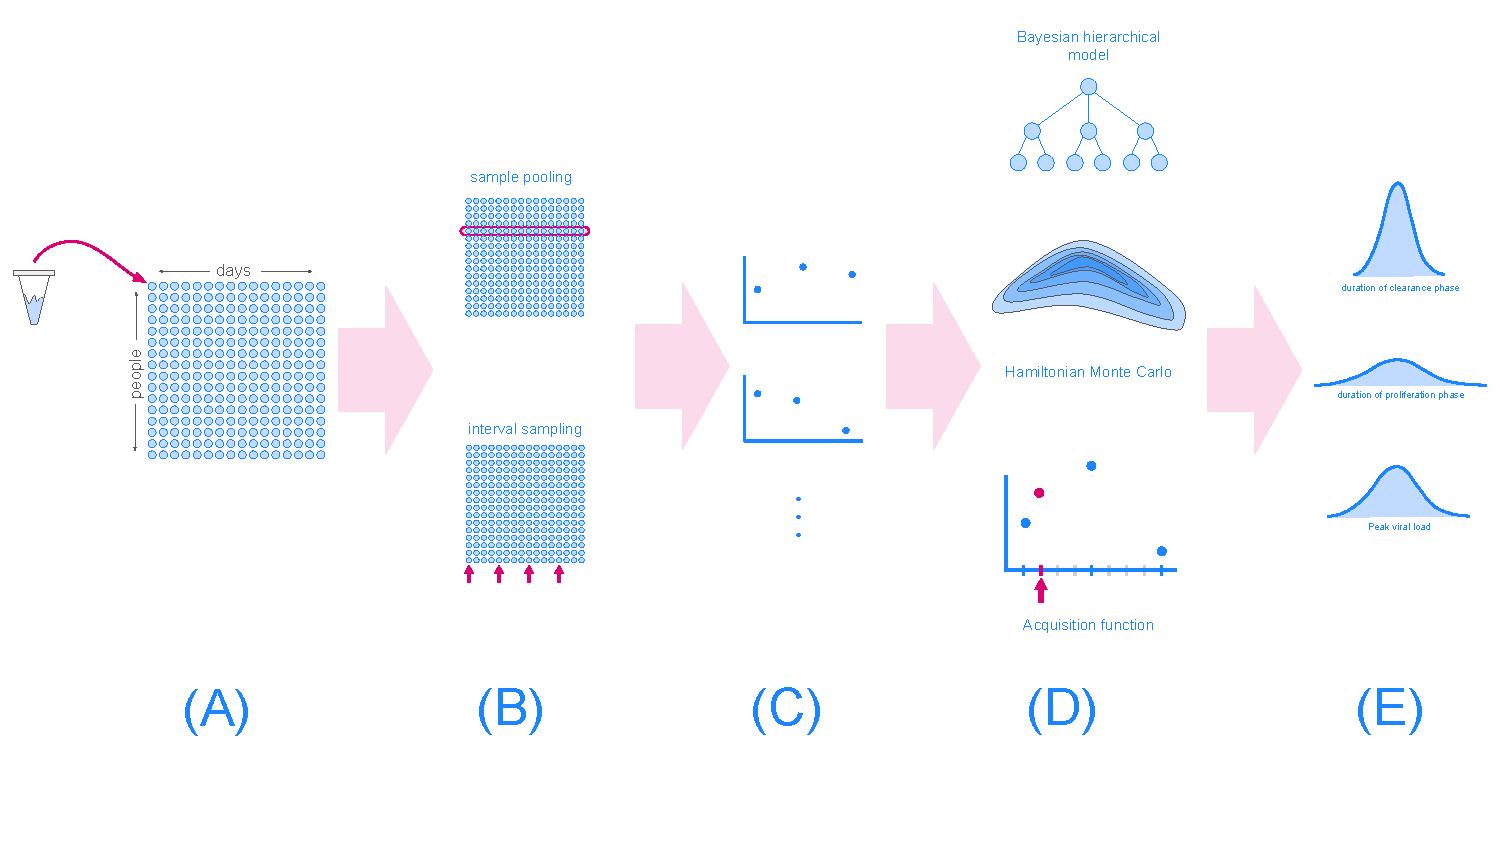
\includegraphics[width=1\textwidth]{../fig/pipeline.pdf}
      \caption{The model fitting pipeline \vlr{(what about adaptive sampling?)}. In Phase (A), subjects provide saliva samples over several
       days to create a matrix of samples with dimensions subjects by days. In Phase (B), sample 
       pooling and interval sampling are used to identify the locations of infections in the 
       matrix. This results in a series of partially sampled viral load trajectories. Using Hamiltonian 
       Monte Carlo, the Bayesian hierarchical model specified in \ref{fig:bhm} is fit to the partially 
       sampled trajectories. The fit model provides probability distributions over possible values of 
       the epidemiological parameters of the pathogen.} \label{fig:pipeline}
       
  \end{figure}

\section{Results}



\subsection{Infection Discovery}

\subsection{Model Fitting}

\begin{figure}
    \centering 
    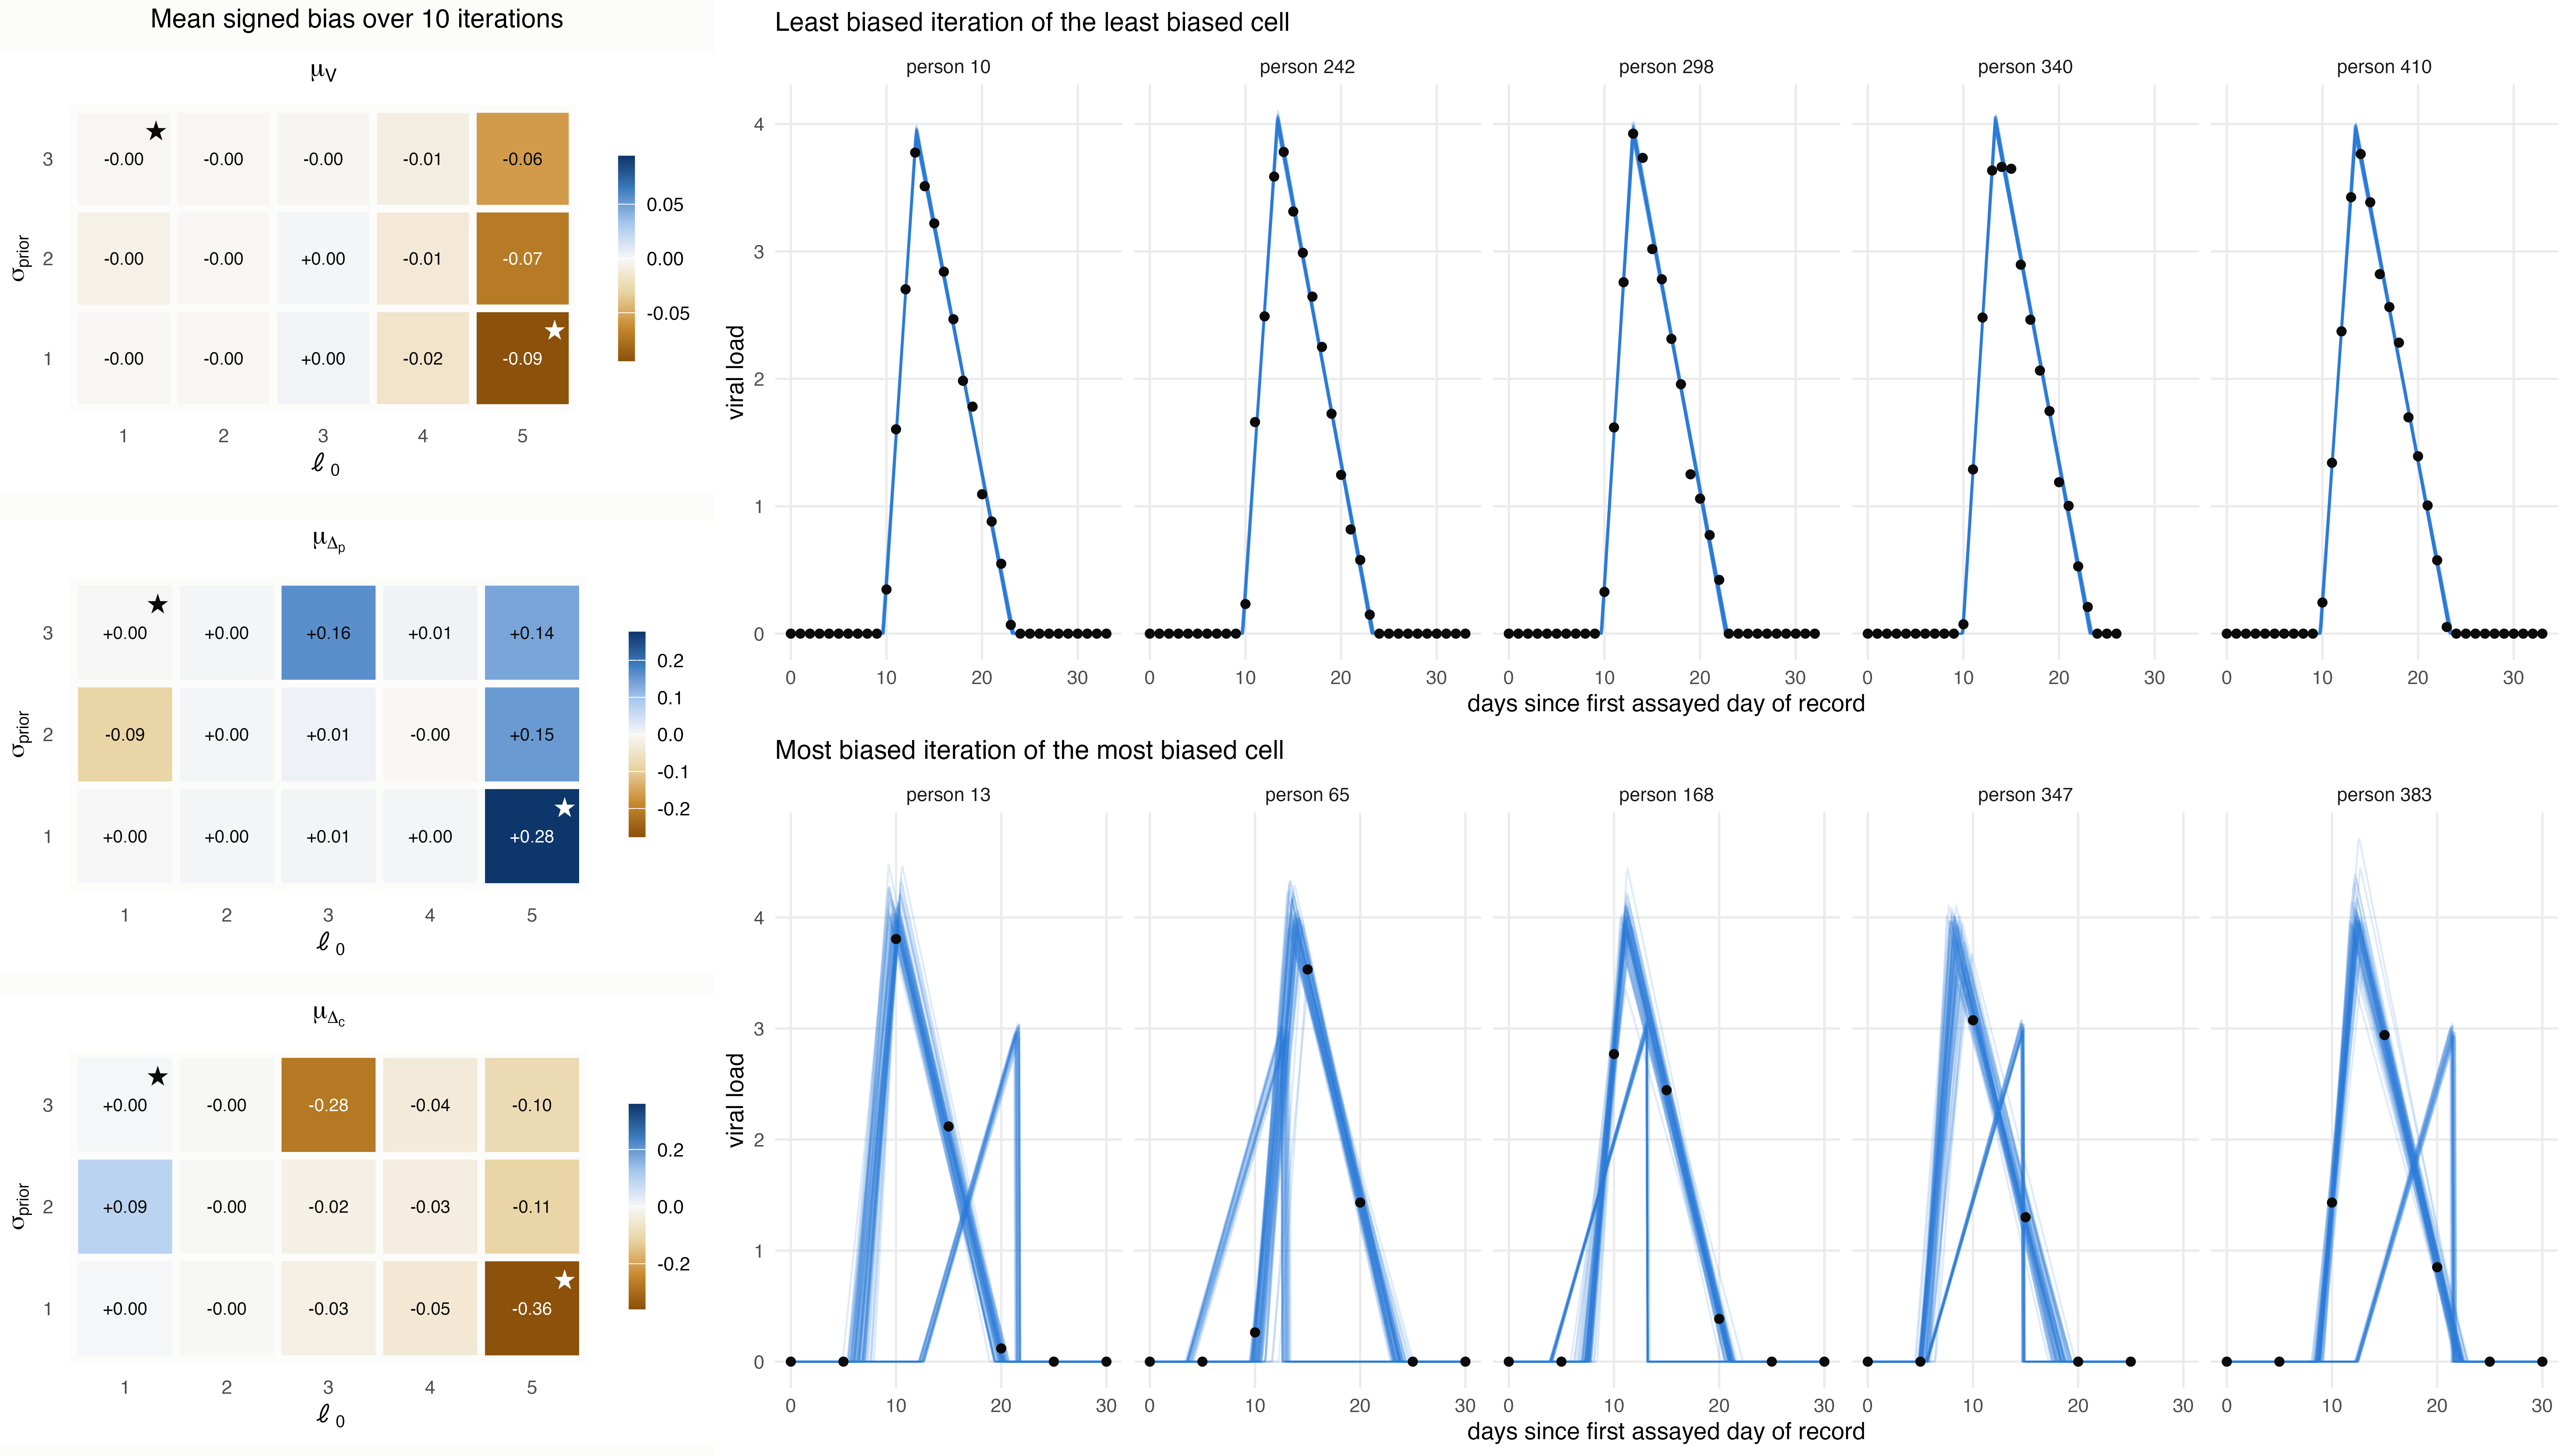
\includegraphics[width=1\textwidth]{../fig/nonadaptive_experiment_plot.png}
    \caption{Performance of fitting the BHM to the outputs of infection discovery.
    For 10 iterations, a synthetic 500 person by 500 day sample matrix is generated.
    Then for 15 combinations of $\sigma_{\text{prior}}$ and $\ell_0$ values, infection discovery is performed and the model is fit to its output.
    The mean signed bias is then averaged over the 10 iterations.
    For the cells with the highest and lowest bias, randomly chosen example infections and a sample of draws from the HMC fitting process are plotted.} \label{fig:nonadaptive_results}
    
\end{figure}

\begin{figure}
    \centering 
    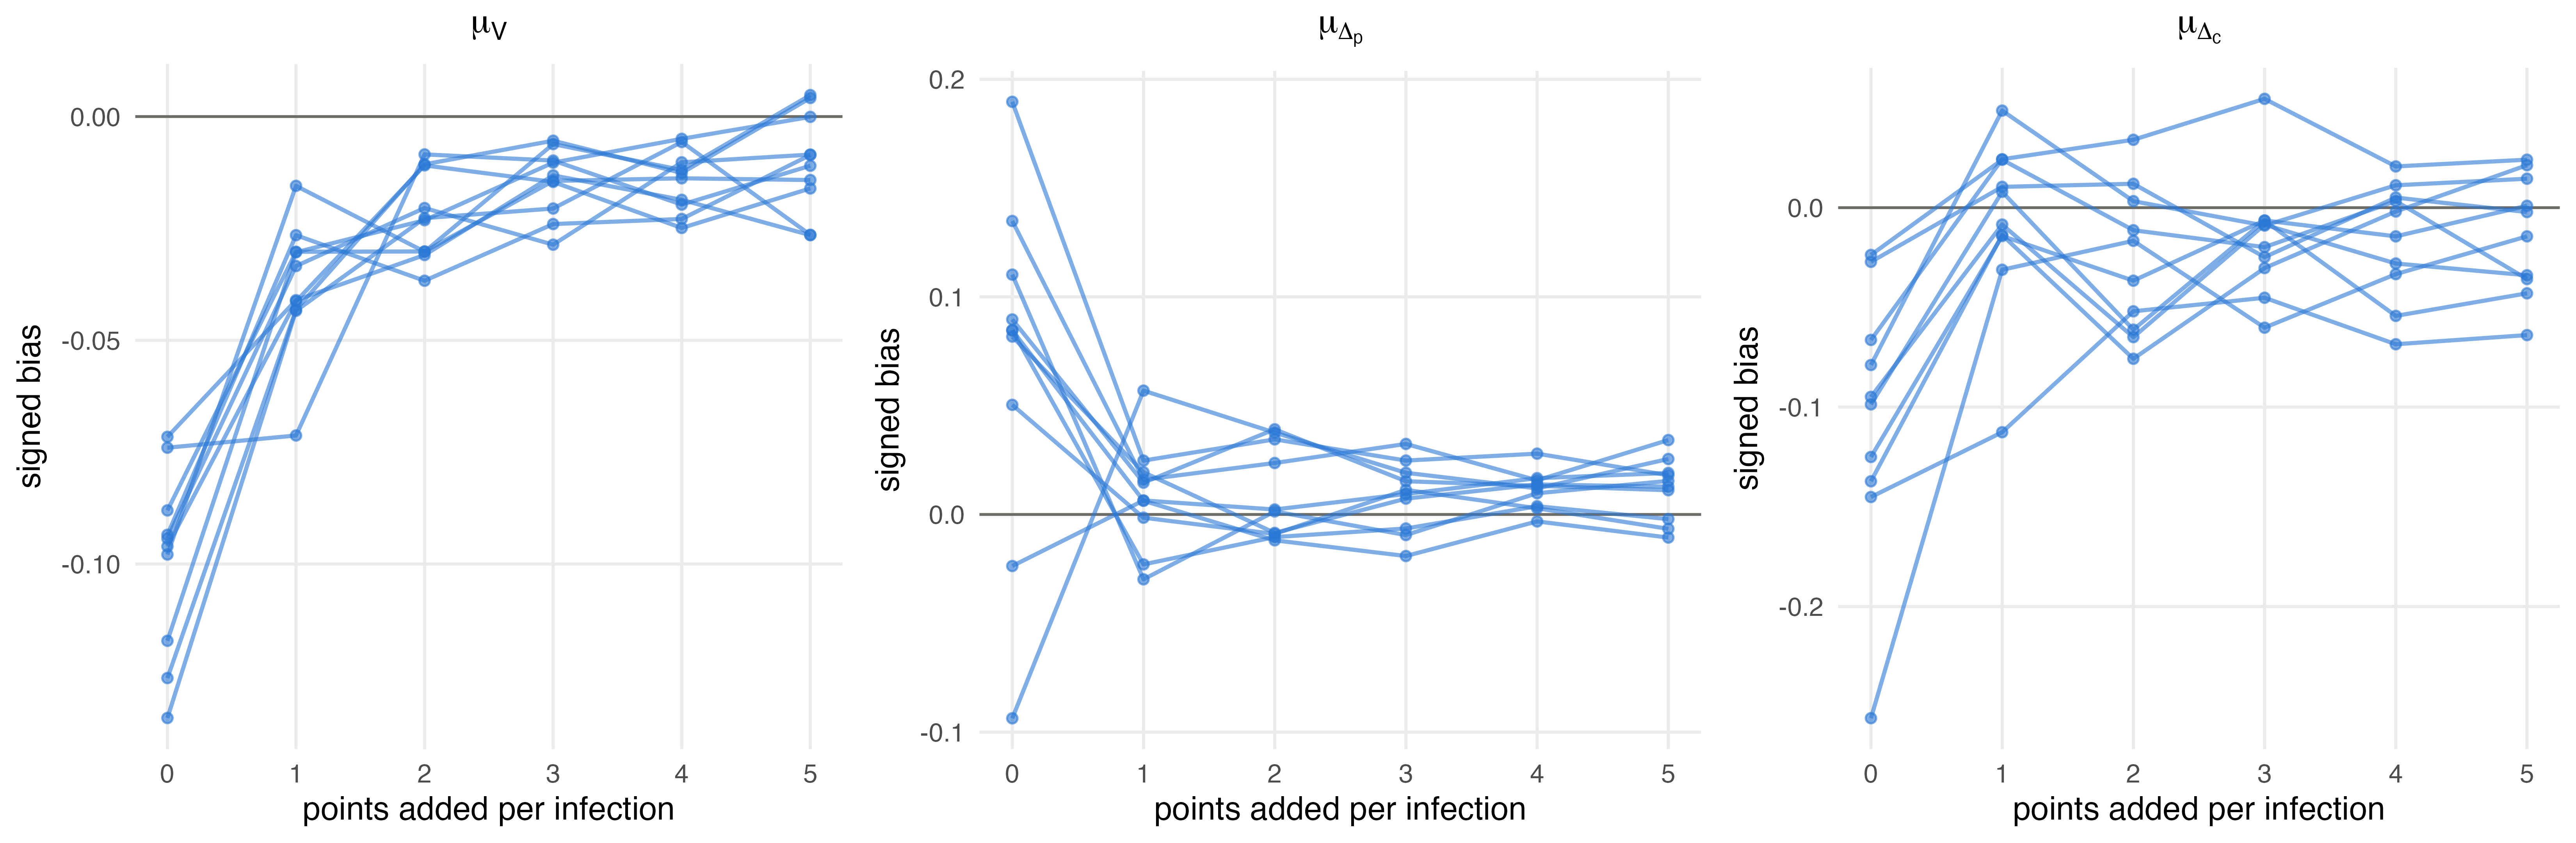
\includegraphics[width=1\textwidth]{../fig/adaptive_worst_cell.png}
    \caption{Impact of point acquisition on bias of parameter estimations.
    10 synthetic 500 person by 500 day sample matrices were generated.
    The following process was performed on each matrix.
    Infection discovery with $\ell_0 = 5$ was performed on the matrix, and the output was fit to the BHM via HMC with all priors having standard deviation 1.
    Then 5 rounds of point acquisition were performed.
    The bias at each point addition step for each of the 10 matrices is plotted for parameters $\mu_V$, $\mu_{\Delta_p}$, $\mu_{\Delta_c}$.} \label{fig:adaptive}
    
\end{figure}



\subsection{Interpreting Error}
We have shown that it is possible to reduce the cost of data collection while maintaining the quality of parameter estimates produced by the resulting model.
Still, if some error is permitted, we can reduce costs even further.
It is therefore important for investigators seeking to optimize sample collection and assaying to develop an understanding of how error scales with respect to their question.
To illustrate this, and to contextualize the error values presented in earlier sections of this paper, we provide the following two case studies.
The first case study concerns a question of pathogen dynamics and statistical power, while the second case study concerns an effort to make optimal public health recommendations.

First, suppose we would like to determine whether, for a given pathogen, the peak viral load is different depending on whether the host is vaccinated.
This case study is inspired by the methodologies employed by Kissler et al. in \cite{kissler2023viral}.
We will investigate this question by collecting longitudinal data from two populations: vaccinated and unvaccinated.
This data will be compiled into a matrix onto which our infection discovery algorithm will be applied. 
The trajectories discovered will then be sorted into two groups: V (vaccinated) and U (unvaccinated).
We will separately fit the BHM to group V and group U, skipping any additional point acquisition.
Then, to determine whether the peak viral loads are significantly different, we will take the difference of the two groups' relevant posterior draws entry-wise.
If less than 5\% of the differences fall on a given side of 0, the peaks of the two groups are considered significantly different.

To investiate the impact of reduced assay rate on an investigator's ability to answer the proposed question, we conducted the following experiment.
We generated a synthetic matrix of infections, where the vaccination status of an individual is determined randomly.
There are two separate models from which we generate the viral kinetics for vaccinated and unvaccinated individuals.
The two models are identical except for the distributions from which peak viral load is drawn, which have different means.
If we assay every sample in the matrix, we can correctly determine that the two groups have different underlying peak viral load distributions.

\begin{figure}
    \centering 
    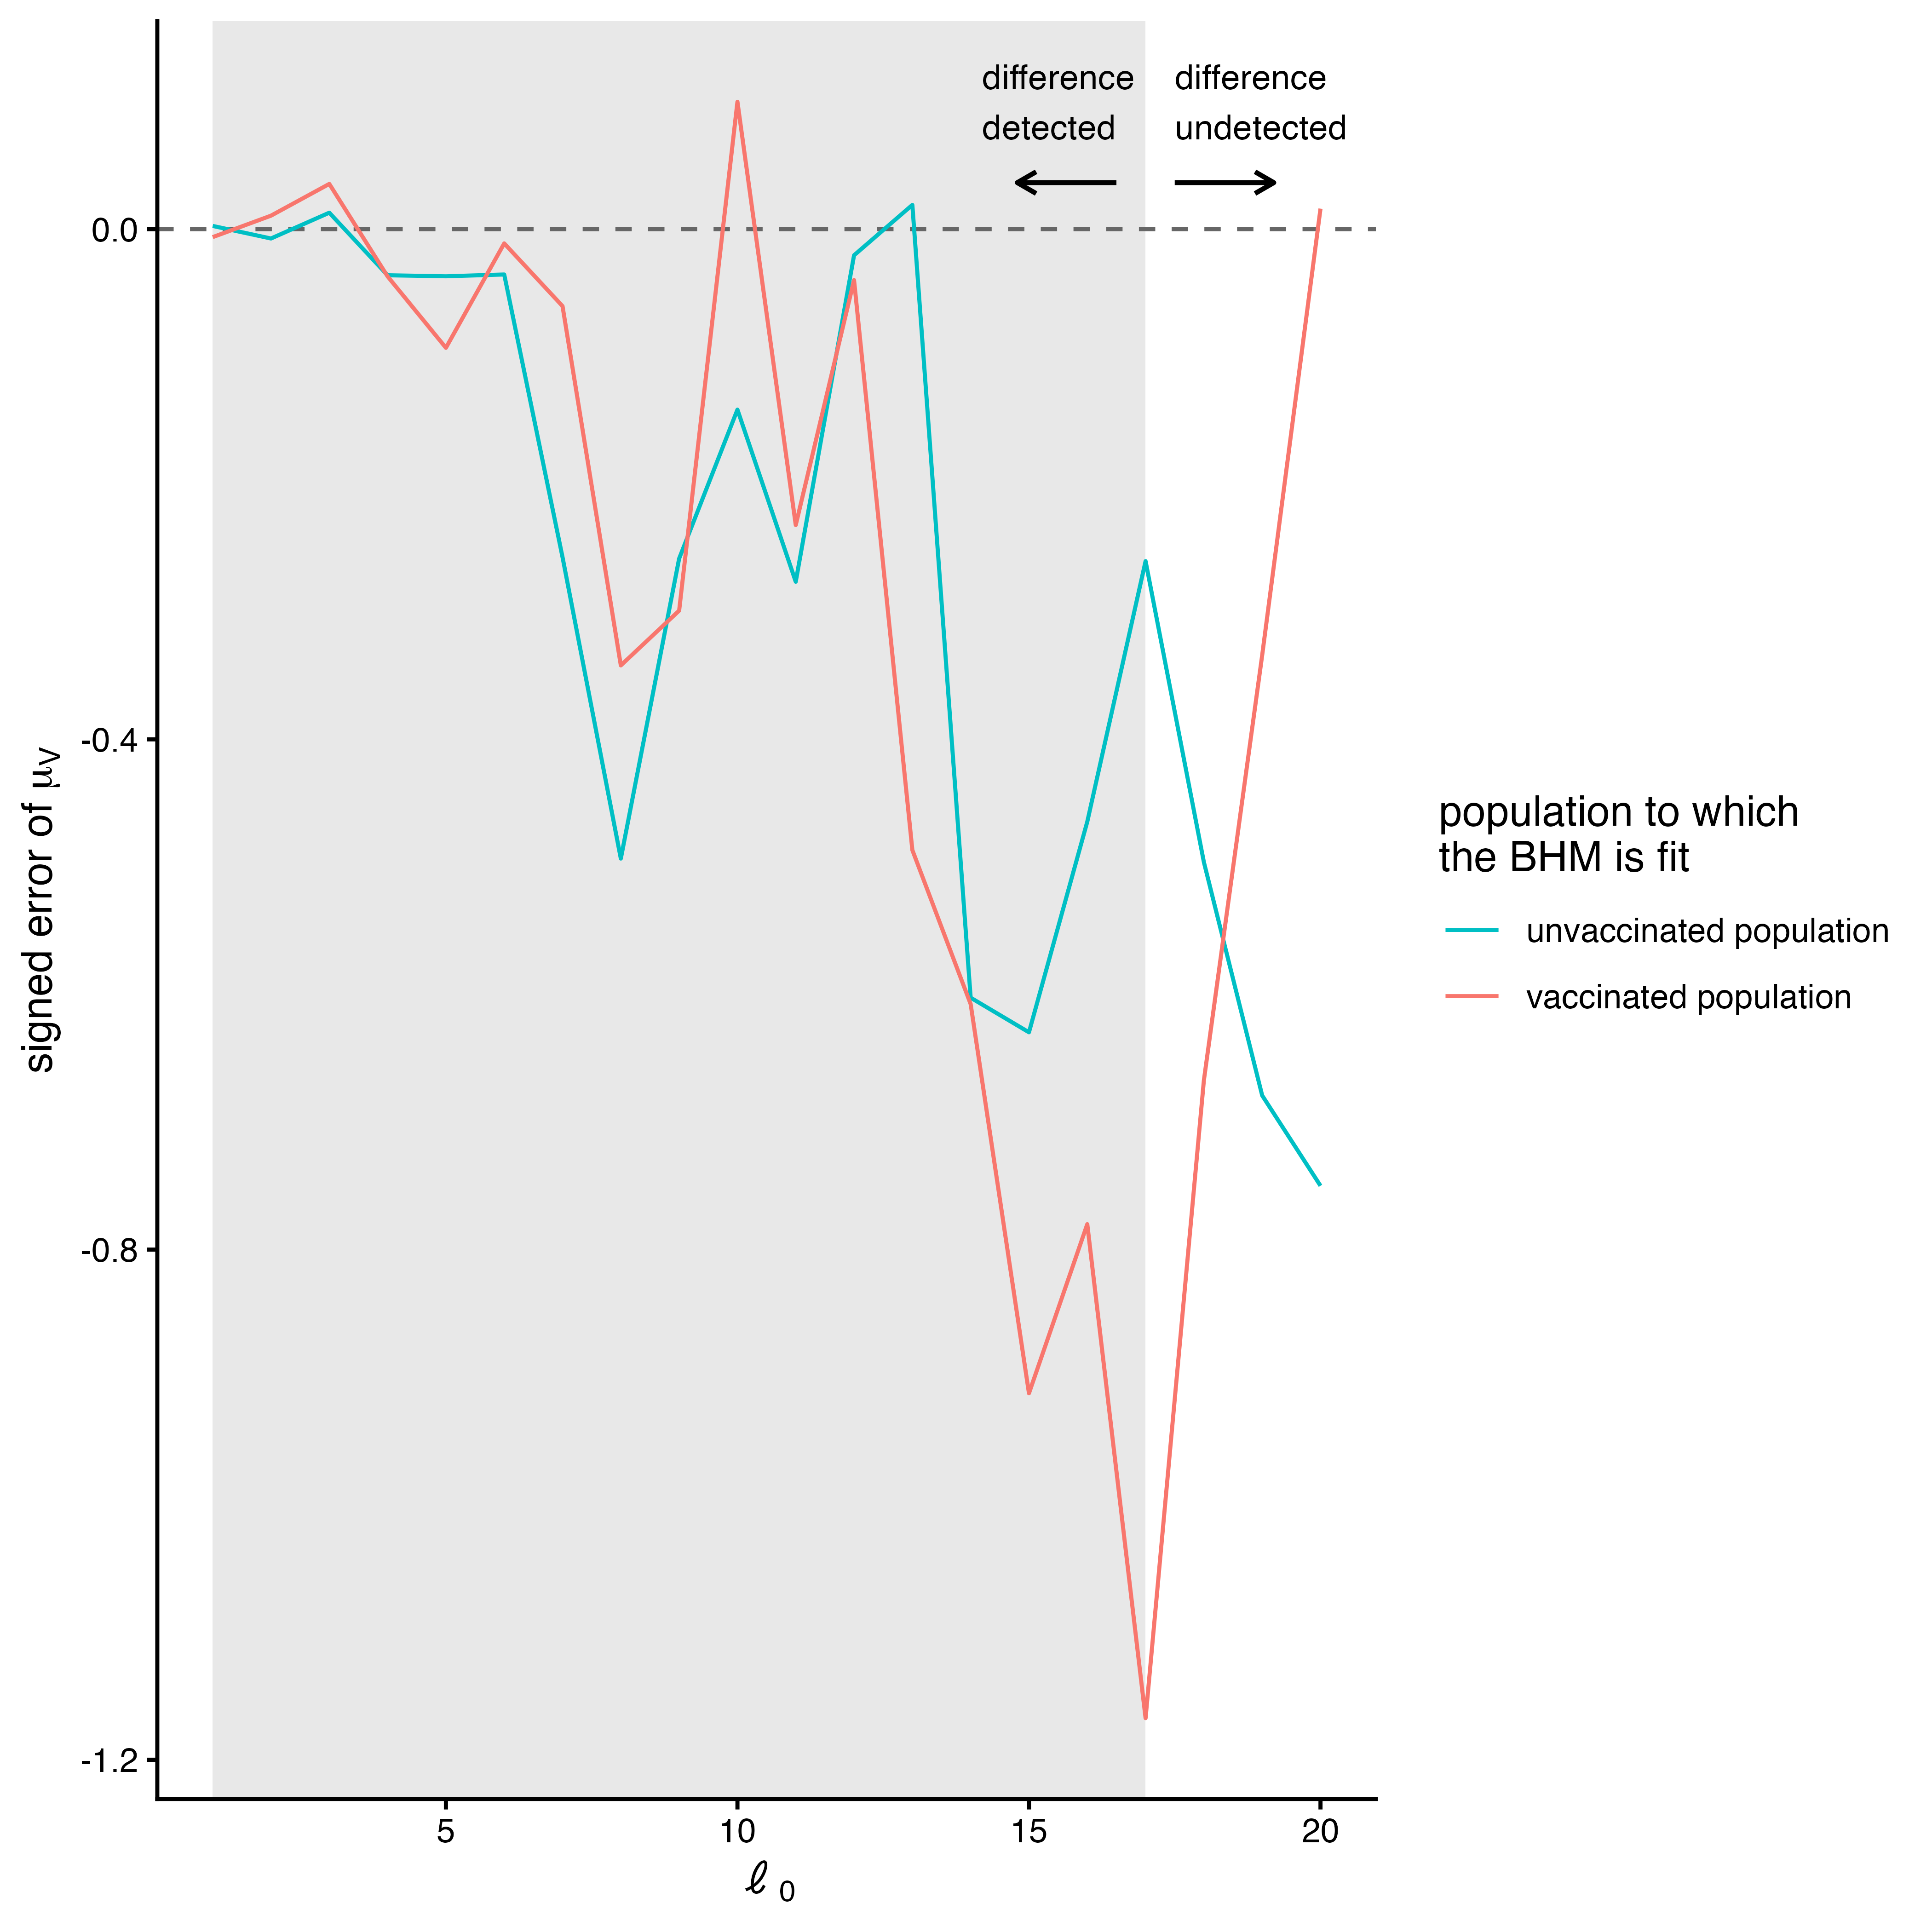
\includegraphics[width=1\textwidth]{../fig/question1.png}
    \caption{Case Study 1.} \label{fig:question1}
\end{figure}


Figure \ref{fig:question1} demonstrates how our ability to identify this difference varies with the interval at which we assay participants.
The complete details of this simulation are available in Appendix [BLAH].
Notably, for values of $\lo$ less than or equal to 6, we are able to correctly detect the difference in the peak viral load distributions of the two groups.
That is, with $1/6$ as many assays, the two groups can still be distinguished.
We also plot the $\beta_1$ RMSE of the two fit models for varying $\lo$.
For some higher $\lo$ values for which the viral load question is correctly answered, the RMSE of the actual parameter estimates are nontrivial.
Therefore, if one wanted to both determine whether unvaccinated and vaccinated populations have significantly different peak viral loads \textit{and} provide accurate estimates of what those peak viral loads are, it would be advantageous to select a smaller sampling interval.
We note, however, that this interval length need not be 1; for $\lo = 3$, the RMSEs of both the model fit to U and the model fit to V are similar to the RMSEs acheived with complete assaying.

This simulation demonstrates that key pathogen kinetics questions can be answered even when the parameter estimates are noisy.
This fact allows for a more extensive reduction in the cost of data collection.
Still, for those questions that require more accurate estimates of epidemiological parameters, costs can be reduced (in this case, by a factor of 3), without sacrificing performance.

In the second case study, we consider the task of selecting the optimal length of isolation for individuals infected with a given pathogen.
To select isolation length, we optimize over testing effectiveness (TE) as defined by Middleton et al. in \cite{BLAH}.
Details on the calculation of TE and the optimization process can be found in Appendix [BLAH].
The value of TE is computed using, among other information, a model of the viral kinetics of the pathogen.

\begin{figure}
    \centering 
    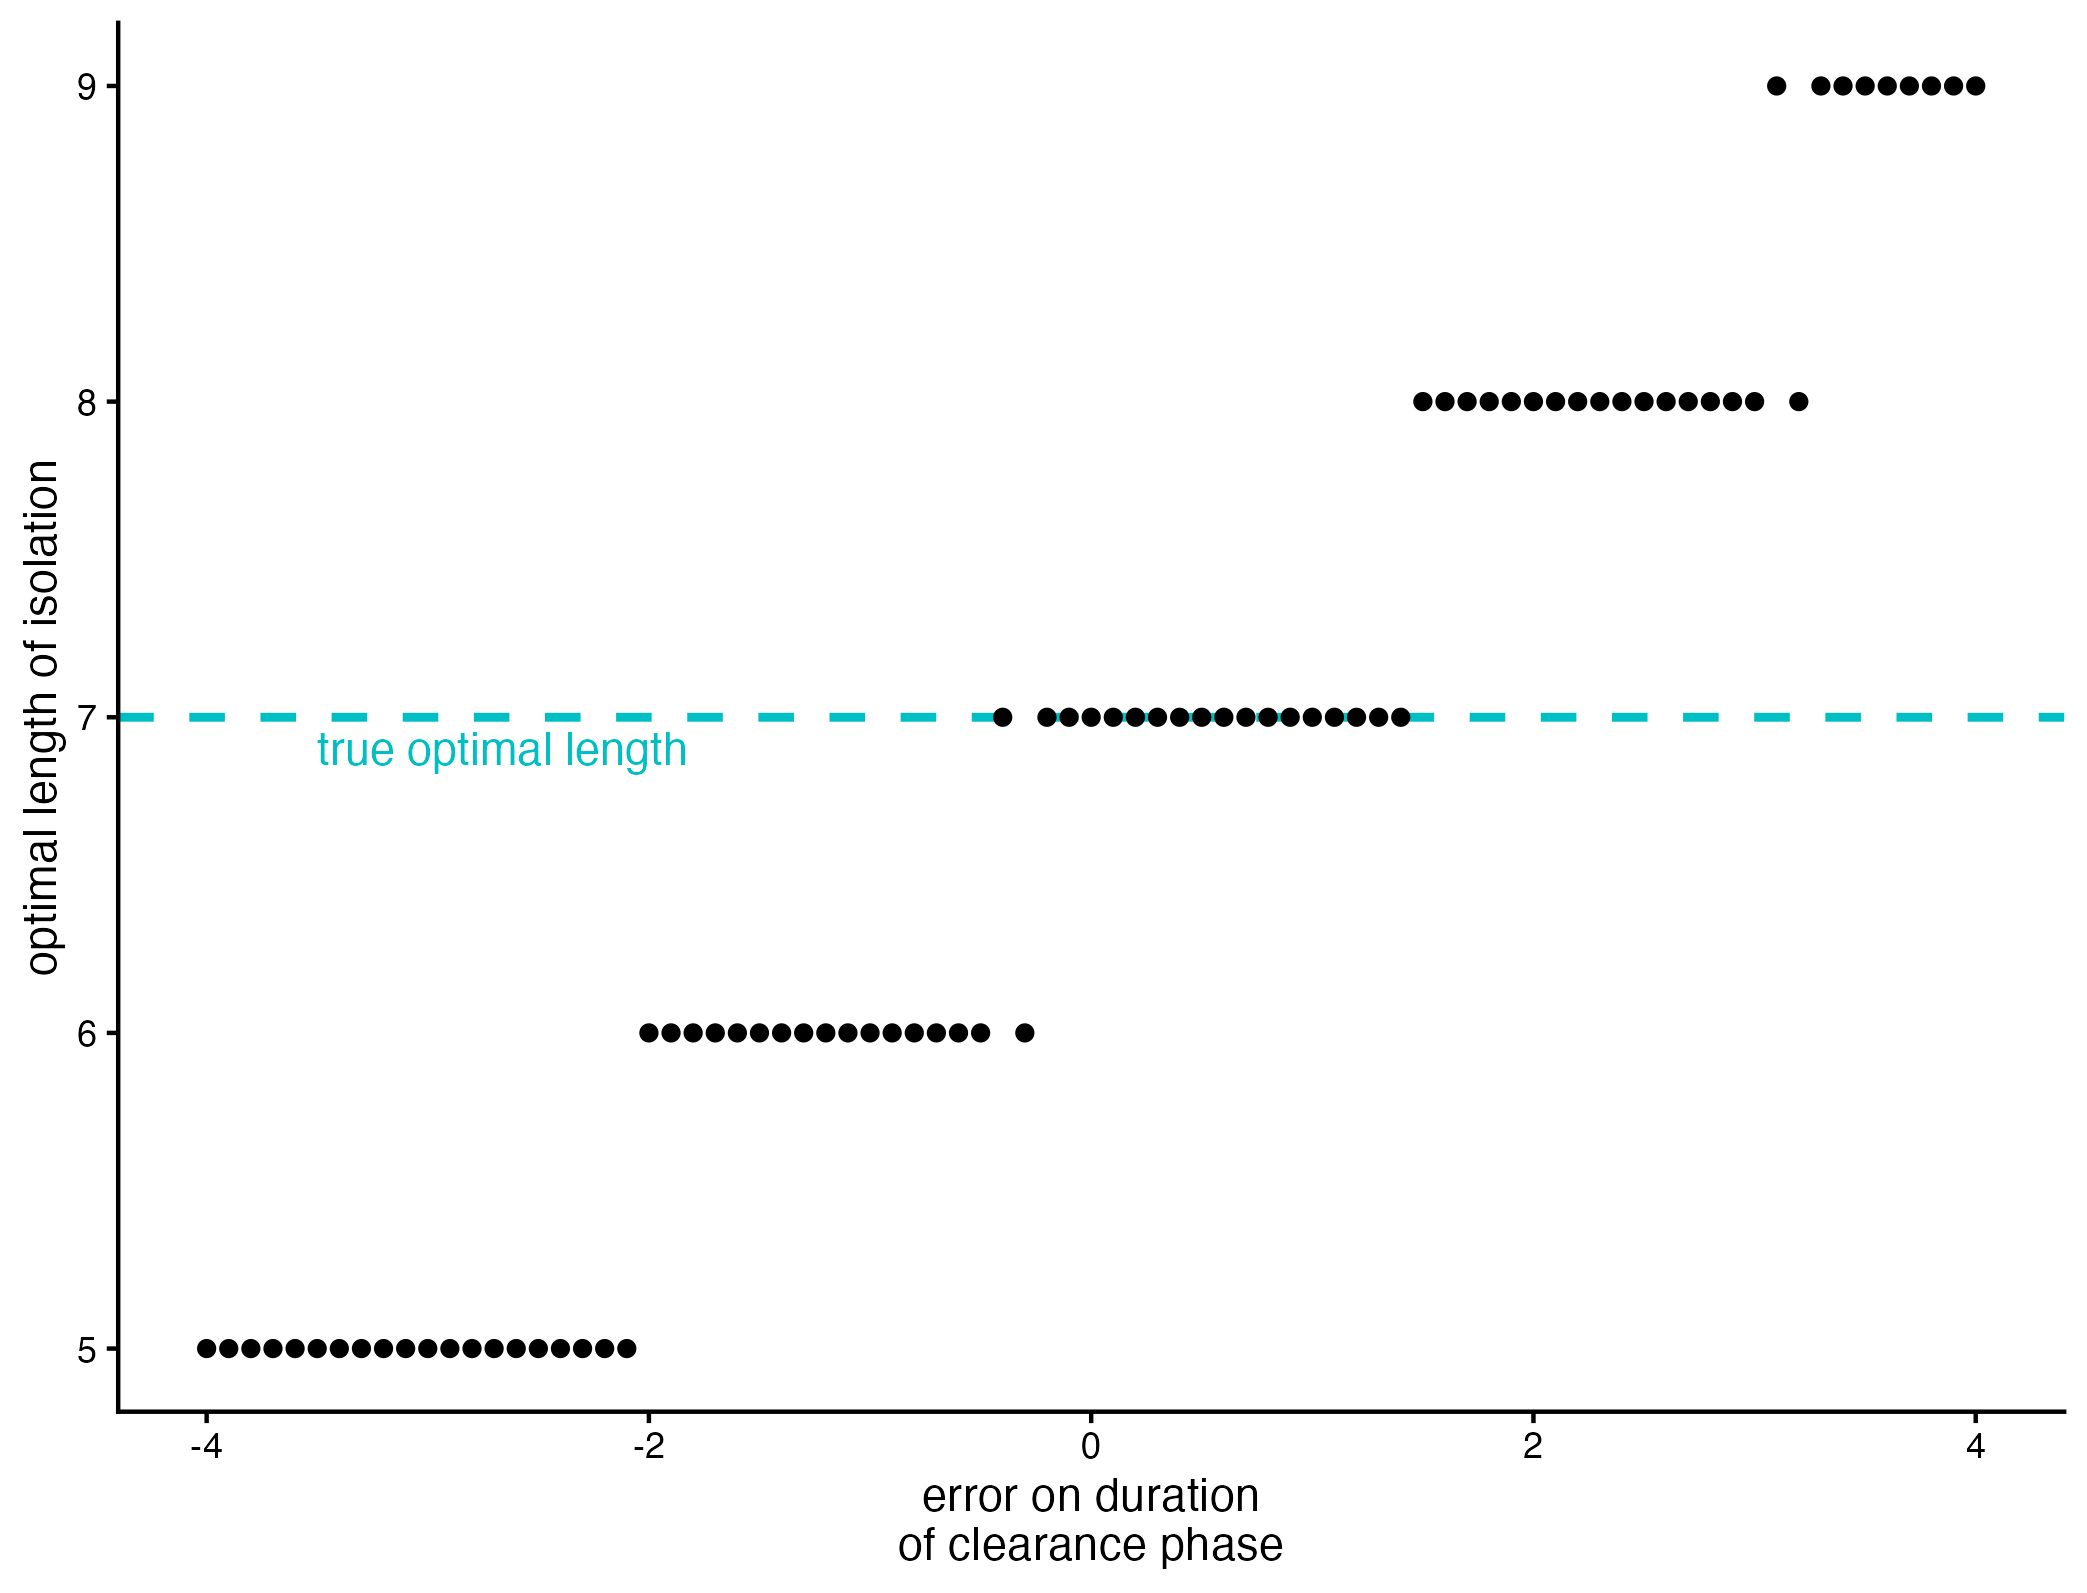
\includegraphics[width=1\textwidth]{../fig/question2.png}
    \caption{Case Study 2.} \label{fig:question2}
\end{figure}

Figure \ref{fig:question2} shows the selected optimal length of isolation for varying amounts of error on the parameter which describes the mean of the clearance phase duration.
This figure highlights the impact of the sign of the error on the isolation recommendation.
Negative error leads to isolation recommendations that are shorter than the true optimal, while positive error generates longer recommended lengths.
Additionally, a lesser magnitude of negative signed error is necessary to alter the recomended length than of positive error.
This brings a key dimension of cost optimization to light — two sampling approaches that cause the same magnitude of error on the parameter estimates, but in opposite directions, may not have the same impact on the researcher's ability to answer their question.
Just as the sign of the error on the clearance phase duration parameter causes varying impacts on the recommended isolation length, the direction in which we erroneously estimate optimal isolation length causes varying public health impacts.
An isolation period that is too short will allow individuals who are still infectious to exit isolation too early, while a longer-than-necessary isolation period may result in an unecessary burden on the infected individual.
Public health officials therefore may allow assaying optimization that biases estimates in one direction, but not the other.

Of course, in the above case studies, we know the correct answer in advance, and can evaluate the performance of optimization efforts by determining whether the undersampled data produces the same result.
When collecting data with the goal of answering a novel question, the researcher must determine the sensitivity of their analysis process to parameter estimate error in advance.

\section{Acknowledgements}
We thank Stephen Kissler for helpful discussions.

\section{Appendix}

\subsection{Accuracy and Cost of Infection Discovery}\label{sec:infx-disc}
For an arbitrary infection $i$ contained in sample matrix $\samplematrix$, the probability the infection discovery algorithm misses $i$ can be expressed as follows.
\begin{equation*}
    \begin{split}
            \prob(\text{miss }i) &= \prob(\li \geq \lo) \prob(\text{miss }i | \li \geq \lo) + \prob(\li < \lo) \prob(\text{miss }i | \li < \lo) \\
            &= \prob(\li < \lo) \prob(\text{miss }i | \li < \lo) \\
            &= \int_{0}^{\lo} \prob(\li) \prob(\text{miss }i | \li) d\li \\
            &= \int_{0}^{\lo} \prob(\li) \left(1 - \frac{\li}{\lo} \right) d\li  \\
            &= \int_{0}^{\lo} \prob(\li) - \int_{0}^{\lo} \prob(\li)\frac{\li}{\lo} d\li  \\
            &= \prob(\li < \lo) - \frac{\prob(\li < \lo)}{\lo} \expec \left[ \li | \li < \lo \right] \\
            &< \alpha - \frac{\alpha}{\lo} \expec \left[ \li | \li < \lo \right]
    \end{split}
\end{equation*}

We now consider the cost of performing infection discovery on $\samplematrix$.
Suppose each assay costs $\assaycost$.
Then the cost of the pooling step of the infection discovery algorithm is $\assaycost \numpeople$.
The cost of the interval sampling step is 

\subsection{Model Fitting}

\begin{figure}
    \centering 
    \includegraphics[width=1\textwidth]{../fig/nonadaptive_experiment_plot_supplementary.png}
    \caption{.} \label{fig:nonadaptive-supplementary}
\end{figure}
\bibliographystyle{unsrtnat}
\bibliography{refs}
\end{document}